\chapter{Základní problematika virtualizace síťových funkcí}
Jak již vyplývá z názvu, tak tato kapitola se zabývá základní analýzou a popisem problematiky spojené s oblastí virtuální síťových funkcí. Budou zde vysvětleny hlavní důvody pro virtualizaci síťových funkcí, základní principy virtualizace, cloud computing a referenční architektura frameworku pro virtualizaci síťových funkcí. Poté budou zmíněny příklady některých dostupných technologii a řešení, které k virtualizaci síťových funkcí lze použít.

Pro lepší pochopení a přehlednost celé této práce zde budou rozlišeny následující pojmy, se kterými se lze také setkat v odborné literatuře a které budou dále v této práci používány. 

\begin{itemize}
\item Síťová funkce (Network function - NF) - Toto je komponenta síťové infrastruktury, která má dobře definované funkční chování, jako například směrování, NAT, Load balancing, Intrusion detection, atd.
\item Virtuální síťové funkce (Virtual network function - VNF) - Je stejná jako NF, ale zde je funkčnost implementována pomocí softwaru a je nezávislá na hardwaru, na kterém běží.
\item Virtualizace síťových funkcí (Network Functions Virtualization - NFV) - Zde se jedná o označení celého konceptu či frameworku.
\end{itemize}

\section{Potřeba virtualizaci síťových funkcí (NFV)}

Produkční vývoj v telekomunikačním průmyslu se tradičně řídil přísnými standardy kvůli stabilitě a kvalitě komunikace. Přestože tento model v minulosti fungoval, tak vedl nevyhnutelně k dlouhým produkčním cyklům, pomalému tempu vývoje a spoléhání se na proprietární či specializovaný hardware. S příchodem výrazné konkurence v komunikačních službách, od rychle postupujících organizací operujících ve velkém měřítku na veřejném internetu, podnítil poskytovatele služeb pro hledat nových způsobů, jak změnit dosavadní způsob produkčního vývoje.

Pro vyřešení toho problému bylo navrženo v publikacích \cite{NFV_paper2012} a \cite{NFV_paper2013} skupinou několika telekomunikačních provozovatelů ETSI řešení ve formě virtualizace síťových funkcí (network functions virtualization). Později vzniklo více projektů zabývající se touto oblastí jako například OPVNF \cite{OPNFV}  Hlavní cíle tohoto řešení jsou zlepšit následující aspekty provozu telekomunikačních sítí:

\begin{itemize}
\item Smíření investičních nákladů – snížení potřeby nákupu jednoúčelových hardwarových zařízení, možnost platby pouze za využité kapacity a snížení rizik přílišného předimenzování kapacit
\item Snížení provozních nákladů – snížení prostoru, napájení a požadavky na chlazení, zjednodušení správy a řízení síťových služeb
\item Urychlení Time-to-market – zkrácení doby pro nasazení nových síťových služeb, chopení se nových příležitosti na trhu, vyhovění potřebám zákazníka
\item Doručit agilitu a flexibilitu – možnost rychle škálovat (rozšiřovat nebo zmenšovat služby) dle měnících se požadavků od zákazníka. Podpora služeb, které mají být dodány pomocí softwaru na libovolném standardním serverovém hardwaru
\end{itemize}

Jak je uvedeno v \cite{NFVState} a \cite{NFVChalanges}, tak celá myšlenka je založena na tom, že dojde k separování softwarové funkcionality v síťových prvcích od proprietárního hardwaru, na kterém běží. To umožní se síťovými funkcemi zacházek jako s klasickými softwarovými aplikacemi, které mohou běžet na standardním komerčně dostupných serverech jenž organizace v současnosti používají. Tím bude zároveň umožněno flexibilní nasazování těchto síťových funkcí a jejich dynamický provisioning. Díky tomu, že jsou síťová funkce odděleny od hardwaru, tak je také možné jejich vhodnější umístění v topologii. To znamená dle požadavků na umístění mohou být nasazeny v datových centrech, síťových uzlech či přímo v uživatelově koncovém bodě. Hlavní koncept virtualizace síťových funkcí znázorňuje obrázek č. \ref{fig:vize_NFV}. 

\begin{figure}[h]
\begin{centering}
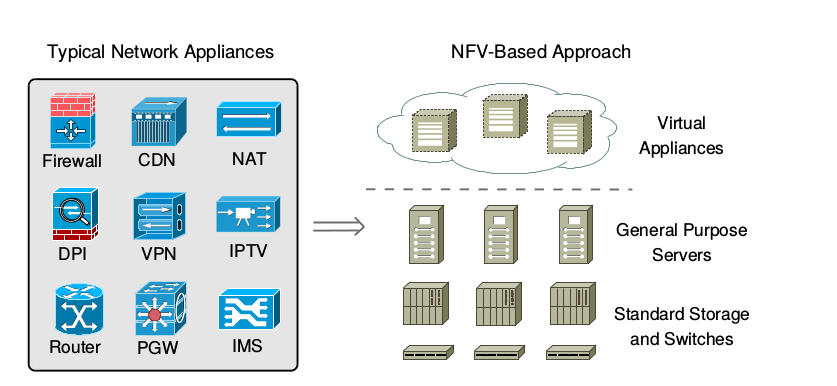
\includegraphics[scale=0.5]{images/vize_NFV}
\par\end{centering}
\caption{Koncept virtualizace síťových funkcí (NFV)\label{fig:vize_NFV}}
\end{figure}

Za zmínění stojí poznámka v \cite{NFVState}, kde je řečeno, že obecný koncept oddělení síťové funkce od hardwaru ještě nutně neznamená potřebu využití virtualizace. Protože budou síťové funkce dostupně jako software, tak mohou být nainstalovány a provozovány přímo na fyzickém stroji. Ovšem rozdíl je, že tento stroj již nebude speciální hardware, ale klasický server. Tento scénář může být do jisté míry použit při nasazovaní síťových funkcí v malém měřítku např. v uživatelských koncových bodech. Avšak pro plné využití všech výše zmíněných výhod, které jsou třeba ve velkých datových centrech, je třeba s použitím virtualizace počítat. To vše umocňuje fakt, že většina datových center v současnosti již využívá cloud computing. 

\section{Základní princip virtualizace}

Základním problém v tradičním modelu IT infrastuktury je, že servery podporují pouze jeden operační systém v čase. Na tomto systému obvykle běží pouze jedna aplikace. Přestože by na tomto systému popř. serveru mohlo běžet více aplikací, tak je lepší držet aplikace odděleně na různých systech z důvodu minimalizace potencionálních bodů selhání. Pokud například nastene s aplikací problém, tak častým řešením je restartování systému. Pokud by na systému bylo více aplikací, znamenalo by to jejich vyřazení z provozu po dobu restartu, který může trvat velice dlouho. \cite{VM_book}

Z výše zmíněných důvodů došlo k velkému rozvoji a nasazování virtualizace. Virtualizací obecně označujeme techniky, které umožňují k dostupným hardwarovým zdrojům přistupovat jiným způsobem, než jakým fyzicky existují. Je tomu díky softwaru, který tento hardware abstrahuje a vytvoří tím virtuální prostředí. Virtualizované prostředí se dá snadněji přizpůsobit potřebám uživatelů, případně skrýt pro uživatele nepodstatné detaily (jako např. rozmístění hardwarových prostředků). Tím je tedy umožněno na jednom fyzickém serveru provozovat více od sebe oddělených virtuálních strojů, které mají každý svůj vlastní operačních systému s aplikacemi. Software pro virtualizaci se nazývá hypervisor.\cite{VM_book}

Jak zmiňuje \cite{VM_architektura}, tak existují tyto dva základní typy hypervisorů:

\begin{itemize}
\item Typ 1 (Nativní) - Tento hypervisor běží přímo na fyzickém hardwaru. Tím umožňuje provozovat více operačních systému na jednom fyzickém stroji. Příkladem takového hypervisoru je VMware ESXi a XEN.
\item Typ 2 (Hostovaný) - Na rozdíl od předchozího případu tento typ hypervisoru běží v prostředí operačního systému. Příkladem je například KVM či Microsoft Hyper-V
\end{itemize}

\begin{figure}[h]
\begin{centering}
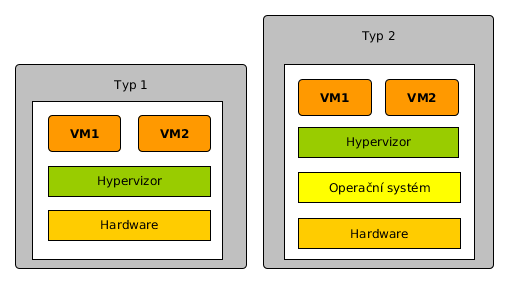
\includegraphics[scale=0.5]{images/virtualization}
\par\end{centering}
\caption{Schéma hypervisorů \label{fig:virtualization}}
\end{figure}

Obrázek \ref{fig:virtualization} zobrazuje schématický popis obou hypervisoru a jejich rozdíl. Problematika virtualizace je velice rozsáhlá a více informací o ní poskytují zdroje \cite{VM_book} a \cite{VM_architektura}.

\section{Cloud Computing}

Jak již bylo zmíněno, tak cloud computing, nebo někdy také označován pouze jako cloud, je oblast, ve které je velký potenciál pro využití virtuálních síťových funkcí. Z tohoto důvodu bude v této části jeho problematika přiblížena.

Cloud je technologie, kterou v poslední době začala provozovat většina větších organizací, jak ukazuje \cite{Cloud_adoption}. Cloud Computing má mnoho definic. Dle definice uvedené v \cite{Cloud_book} ho lze charakterizovat jako poskytování služeb, programů a výpočetních zdrojů servery dostupnými z internetu s tím, že uživatelé k nim mohou přistupovat vzdáleně.

Z technického hlediska tvoří cloud veškeré služby poskytované přes Internet a zároveň i infrastruktura, která tyto zdroje poskytuje. Tuto infrastrukturu tvoří velké množství fyzických serverů, které jsou vzájemně propojeny. Na těchto serverech běží hypervisor, který vytvoří virtuální infrastrukturu. Pro vytváření cloudových služeb zde musí ještě existovat cloudová platforma, která dokáže celou tuto virtuální infrastrukturu spravovat. \cite{Cloud_book}

Dle \cite{Cloud_book} existuje 5 základních atributů, kterými se cloud computing vyznačuje. Jsou to tyto:

\begin{itemize}
\item Služby dostupné na požádání
\item Všudypřítomný síťový přístup
\item Sdílení zdrojů
\item Vysokou elasticitu
\item Měření využitých zdrojů
\end{itemize}

\subsection{Distribuční modely}

Dle \cite{CloudSurvey} lze cloudové služby lze rozdělit do 3 základních kategorii. V \cite{NFV_use_cases} jsou k těmto kategorii přiřazeny příklady užití z oblasti virtualizace síťových funkcí. 

\begin{itemize}
\item Infrastracture as a Service (IaaS) - Nejzákladnější  model  poskytování  cloudových  služeb. IaaS cloudové platformy nabízejí například výpočetní výkon, virtuální disky, blokové a souborové úložiště či virtuální sítě.  Poskytovatelé  IaaS  cloudových  platforem  poskytují tyto zdroje na vyžádání ze svých datových center. Toto je možné díky skupiny hypervisorů v rámci cloudu, které mohou provozovat velké množství virtuálních strojů  a  mají  schopnost  škálovat  poskytované  služby v  závislosti  na  měnících  se požadavcích přicházejících od zákazníků. Tento model může tedy sloužit i pro poskytnutí všech potřebných zdrojů celé infrastruktury pro virtualizaci síťových prvků, neboli Network Function Virtualization Infrastrakture as a Service. Zde má uživatel pod nejvíce možností, jak navrhnout a spravovat virtuální síťové funkce, protože v zásadě dokáže nasazovat i vlastně navržené síťové funkce a nejen ty, které mu poskytuje provozovatel cloudu.
\item Platform as a Service (PaaS) - V  modelu  Platforma  jako  služba  (PaaS)  hostují  poskytovatelé cloudových  služeb určitou počítačovou  platformu, kterou následně poskytují koncovým uživatelům přes Internet. Tato platforma většinou bývá prostředí nějakého operačního systému, prostředí  pro  běh  určitého programovacího  jazyka,  databáze  a  webový  server.  Vývojáři  aplikací tím pádem  mohou provozovat a případně vyvíjet svá softwarová řešení bez výrazných nákladů a složitého nákupu a konfiguraci potřebného hardwaru a softwaru. Některé PaaS platformy nastavuje výpočetní  a  úložné  prostředky  aplikace  automaticky  tak,  aby  odpovídala  aktuálním požadavkům aplikace bez nutnosti zásahu zákazníka. NVF v tomto modelu může nabízet síťové služby, které se mohou skládat z více virtuálních síťových funkcí, neboli Virtual Network Platform as a Service. Zde je poskytnuta uživately velká kontrola nad konfigurací a ovládáním celé platformy.
\item Software as a Servicec (SaaS) - V modelu SaaS provozují poskytovatelé cloudových služeb aplikační software v cloudu a uživatelé  k  tomuto  softwaru  přistupují  pomocí  klientského  software  (např.  webové prohlížeče). Uživatelé  cloudu tedy  nespravují infrastrukturu  ani platformu, kde aplikace běží.  Není  proto  třeba zde nic instalovat  a  spouštět  aplikace  na  vlastních  počítačích uživatele, což velmi zjednodušuje údržbu. Cloudové aplikace se liší od ostatních aplikací v možnostech  škálování, kterého  může  být  dosaženo  díky  distribuci  úkolů  na  více virtuálních strojů, a tím reagovat na měnící se poptávku. Tento proces je pro uživatele služby transparentní, uživatel vidí pouze jeden přístupový bod pro danou aplikaci. Do této kategorie služeb může patřit poskytování virtuálních síťových funkcí, která je pouze ve formě softwarové aplikace, neboli VNFaaS. Takovéto aplikace poskytují síťovou funkci pro síťové správce a uživatele nejčastěji v privatním cloudu. 
\end{itemize}

\subsection{Modely nasazení}

Existuje několik základních modelů nasazení cloud computingu resp. cloudových platforem, které uvádí \cite{CloudSurvey}. V \cite{NFV_use_cases} lze k nim opět najít určité příklady z oblasti virtualizace síťových funkcí.

\begin{itemize}
\item Privátní cloud - Privátní cloud je  infrastruktura  provozována  výhradně  v  rámci  jedné  organizace. Může být spravován interně nebo prostřednictvím třetí strany a hostování může být opět interní nebo externí.  Aby  mohl  podnik  využít  privátní  cloud,  musí  nejprve  navrhnout a uzpůsobit k tomuto účelu svoji stávající infrastrukturu, která musí být virtualizována.  Vlastní  přechod  vyvolává  řadu  bezpečnostních  otázek,  které  je třeba řešit, aby se zabránilo vážným zranitelnostem celého řešení. Privátní cloud je přesně ten typ modelu, kde lze najít využití pro virtualizaci síťových funkcí.
\item Veřejný cloud - Veřejné cloudové jsou cloudové služby, jako jsou aplikace, výpočetní výkon, úložiště a další, které jsou k dispozici široké  veřejnosti.  Služby  jsou  poskytovány  zdarma  nebo  podle modelu  platby  za  množství  použitých  služeb.  Je  zvykem,  že  veřejní  poskytovatelé cloudových  služeb,  jako  je  Amazon  AWS,  Microsoft  nebo  Google,  vlastní  a  provozují hardwarovou infrastrukturu a nabízejí k ní přístup pouze přes Internet. V tomto modelu není očekáváno využívání NFV.
\item Hybridní cloud - Hybridní  cloud je  spojení  dvou  nebo  více  cloudů  (soukromých,  komunitních  nebo veřejných),  které  zůstávají  samostatné,  ale  jsou  těsně  propojeny.  Toto  složení  rozšiřuje možnosti  nasazení  cloudových  služeb  a  tím  umožňuje  IT  organizacím  využít  veřejné cloudové prostředky k uspokojení dočasných potřeb. Tato schopnost umožňuje hybridním cloudům škálovat přes více nezávislých cloudů. V tomto modelu může být využito NFV především na straně soukromého cloudu.
\item Komunitní cloud - V rámci komunitního cloudu sdílí infrastrukturu cloudu několik organizací, které mají společné zájmy (bezpečnost, dodržování předpisů, působnost, atd.). Komunitní cloud může být spravován interně nebo prostřednictvím třetí strany. Náklady jsou rozloženy mezi méně uživatelů než na veřejném cloudu. V tomto modelu může být využito NVF, pokud se provozovatelé takovéhoto cloudu domluví. 
\end{itemize}


\section{Souvislost NFV a SDN} \label{sub:SDN}

Softwarově definované sítě (SDN) je další z nových technologii, která se snaží vylepšit a automatizovat správu stávajících počítačových sítí. Dle \cite{SDN_clanek} jde o koncept, ve které je oddělena řídící logika (control plane) z jednotlivých routerů a switchů, které přeposílají traffic (data plane). Tím, že dojde k oddělení datové a řídící vrstvy, se routery a switche stanou pouze přeposílající data a veškerá řídí logika může být implementována v jednom logicky centrálním místě (SDN Controller). Z tohoto centrálního místa lze do jednotlivých routerů a switchů předávat instrukce pomocí aplikačních programovacích rozhraní (API). Samotný SDN Controller také obsahuje API, které mohou využívat aplikace a tím řídit, resp. programovat celou počítačovou síť.

\begin{figure}[h]
\begin{centering}
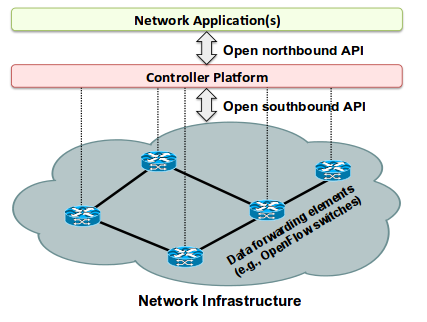
\includegraphics[scale=0.60]{images/SDN}
\par\end{centering}
\caption{Schéma SDN, převzato z \cite{SDN_clanek}\label{fig:SDN}}
\end{figure}

Obrázek č. \ref{fig:SDN} úkazuje jednoduché schéma softwarově definovaných sítí. Celou architekturu lze tedy rozdělit do 3 logických vrstev, které spolu komunikují pomocí API. 

\begin{itemize}
\item Aplikační vrstva - Na této úrovni se nachází samotné síťové aplikace jako jsou například DHCP, ACL, NAT, DNS a další. Jejich vytváření by
mělo být poskytováno prostřednictvím nižší vrstvy, nazývané northbound API.
\item Northbound APIs - Toto API využívají aplikace pro komunikaci s SDN controllerem. 
\item Control vrstva - V této vrstvě je centralizována veškerá logika, které dříve byla v síťových prvcích.
\item Southbound APIs - Jedná se o skupinu API protokolů, které pracují mezi vrstvou infrastruktury a control vrstvou. Jejím hlavním úkolem je komunikace, která povoluje SDN controleru instalovat na samotné síťové prvky rozhodnutí definované v aplikační vrstvě.
\item Vrstva infrastruktura - Nejnižší vrstvou je samotný hardware pro předávání datagramů na fyzické úrovni. Pro funkčnost celé architektury je nutné, aby zde byla nasazena zařízení, která umí přijímat pokyny od control plane skrze southbound API.

\end{itemize}


Přestože Softwarově definované sítě a virtualizace síťových funkcí jsou dvě různé technologie a koncepty, tak se navzájem se doplňují. Fakt, že SDN umožňuje programaticky ovládat počítačovou síť, lze využít pro poskytnutí programovatelné konektivity mezi jednotlivými virtuálními síťovými funkcemi. Naopak SDN může využít NFV tím, že implementuje potřebné síťové funkce jako software. Může tak virtualizovat SDN Controller, který tak může běžet na co nejvhodnějším místě v datovém centru. Je vidět, že tyto dvě technologie se dobře doplňují, proto jsou často součástí jednoho řešení. \cite{SDN_book}


\subsection{Service Chaining}

Jednou z výhod NFV je možnost využít Service Chaining. Service chaining je ve skutečnosti součást SDN. Jde o princip jakým lze dynamicky pospojovat jednotlivé VNF a ovladat tak toky v síti. \cite{SDN_book}

Service chaining není ve skutečnosti nic nového. V klasických počítačových sítích je používán také, ale pomocí fyzických síťových prvků. Jedná se zjednodušeně o způsob zapojení mezi jednotlivými síťovými prvky (či VNF) a způsob, jakým na sebe navazují. Příklad takového zapojení je vidět na obrázku č. \ref{fig:service_chaining}. Zde se provozovatel sítě rozhodl, že odchozí data z klientských stanic musí jít přes firewall, IDS a nakonec přes NAT do Internetu. Příchozí data mají logicky obrácené pořadí. Toto zapojení funguje dobře pro síť, kde není třeba rozlišovat cestu jakou proudí data jednotlivých uživatelských stanic. Ale není to optimální řešení pro sítě s více uživateli, kde každý požaduje jinou síťovou funkci. Potřeba jednotlivých síťových služeb se samozřejmě může v čase měnit. Příklad takové sítě lze nalézt ve většině datových center. 

\begin{figure}[h]
\begin{centering}
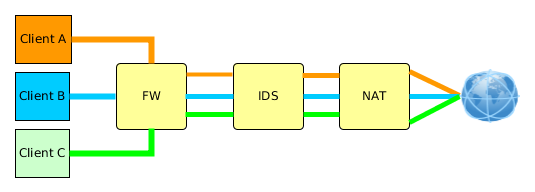
\includegraphics[scale=0.55]{images/service_chaining}
\par\end{centering}
\caption{Ukázka klasického service chainigu pomocí fyzických síťových prvků\label{fig:service_chaining}}
\end{figure}

Zde tedy přichází na řadu VNF spolu s SDN. Protože jednotlivé VNF existují jako virtuální stroje, tak mohou být dynamicky nasazovány dle aktuálním požadavků jednotlivých klientů a pomocí SDN mohou být tyto VM dynamicky pospojovány. Obrázek č. \ref{fig:service_chaining_new} ukazuje schéma zapojení, kde každý klient může mít jinou požadovanou cestu do internetu. Je možná i varianta, kde každý klient má své vlastní VNF s jinou konfigurací.

\begin{figure}[h]
\begin{centering}
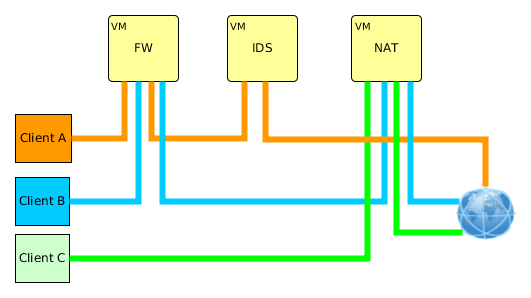
\includegraphics[scale=0.55]{images/service_chaining_new}
\par\end{centering}
\caption{Ukázka VNF service chainigu\label{fig:service_chaining_new}}
\end{figure}

\section{Architektura NFV a VNF} \label{sub:architektura}

V předchozí sekci byla popsána myšlenka a motivace související s virtualizací síťových funkcí. Protože cílem této práce je navržení jednoduchého NFV frameworku, tak je nejprve nutné se seznámit s jeho obecnou architekturou. V této práci se bude vycházet z referenční architektury NVF \cite{NFV_architektura}, která byla navržena organizací ETSI. Jedná se pouze o funkční návrh bez náznaků konkrétní implementace. Od této skupiny existují i podrobnější návrhy jednotlivých částí celého NFV frameworku, které v této práci budou také popsány v příslušných kapitolách.

\begin{figure}[h]
\begin{centering}
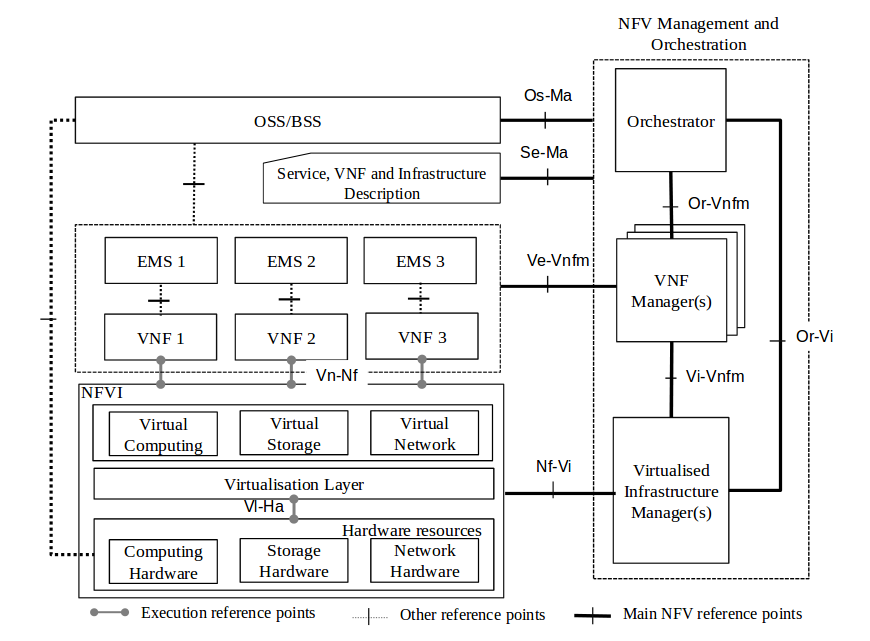
\includegraphics[scale=0.5]{images/NFV_architektura}
\par\end{centering}
\caption{NFV architektura, převzato z \cite{NFV_architektura}\label{fig:NFV_architektura}}
\end{figure}

Jak je vidět na obrázku č. \ref{fig:NFV_architektura}, tak celá architektura se dá rozdělit na tyto 3 hlavní části:

\begin{itemize}
\item Infrastruktura virtualizace síťových funkcí (NFVI) - Jsou všechny softwarové a hardwarové zdroje potřebné k vytvoření prostředí, ve které mohou být jednotlivé VNF být nasazeny. Tato infrastruktura může být velice rozsáhlá, proto je její součástí i síť poskytující konektivitu mezi vzdálenými lokacemi infrastruktury.\cite{NFV_terminology}
\item Virtualizované síťové funkce (VNFs) - Jsou softwarové implementace síťových funkcí, jako je např. NAT a routing. které mohou být nasazeny na NFV infrastruktuře.
\item Management a orchestrace NFV (NFV-MANO) - zde se jedná o řízení softwarových a hardwarových zdrojů v celé infrastruktuře NFV a životního cyklu jednotlivých virtuálních síťových funkcí. Tato část se tedy zaměřuje na řízení a správu všech úloh související v virtualizací v NFV frameworku. \cite{NFV_terminology}
\end{itemize}

Tyto funkční bloky se ještě dále dělí, proto dále v této práci budou tyto jednotlivé části popsány podrobněji a současně k nim budou uvedeny různé možnosti řešení.

\subsection{Infrastruktura NFV}

Ve zdroji \cite{NFV_infrastructure}, který detailně popisuje infrastrukturu pro virtualizaci síťových funkcí (NFVI), je uvedeno, že je v ní sdružení všech základních zdrojů potřebných pro běh virtuálních síťových funkcí (VNF). Z tohoto důvodu sem patří veškerý hardware. Do NFVI také patří některé softwarové komponenty, které jsou společné mnoho VNF a poskytují funkcionalitu potřebnou pro podporu nasazení, propojení či managementu VNF. Celou infrastrukturu může tvořit jeden či více strojů, které mají tyto potřebné funkce. Tyto stroje také mohou být umístěny v různých spolu spojených lokacích. 

Pro zjednodušení lze celou NFV infrastrukturu rozdělit do 3 následujících domén:

\begin{itemize}
\item Compute Domain - Do této domény patří veškeré hardwarové zdroje jako jsou servery, úložiště a komponenty, které tyto zdroje obsahují, např. procesory, pevné disky, síťové karty, atd. Zároveň je zde řešen návrh fyzické topologie. \cite{NFV_compute}
\item Hypervisor Domain - Toto je doména, které představuje softwarové prostředí abstrahující hardware v compute doméně a poskytuje je jako virtuální zdroje. Tyto zdroje následně mohou využívat virtuální síťové funkce. \cite{NFV_hypervisor}
\item Infrastructure Network Domain - V této doméně je řešeno veškeré propojení výše zmíněných domén. Tedy fyzické i virtuální infrastruktury.\cite{NFV_network}
\end{itemize}

Funkci obsaženou v jednotlivých doménách znázorňuje obrázek č. \ref{fig:infrastruktura}. Více informací na tuto problematiku lze nalézt v \cite{NFV_infrastructure} a ve zdrojích uvedených u každé domény. 

\begin{figure}[h]
\begin{centering}
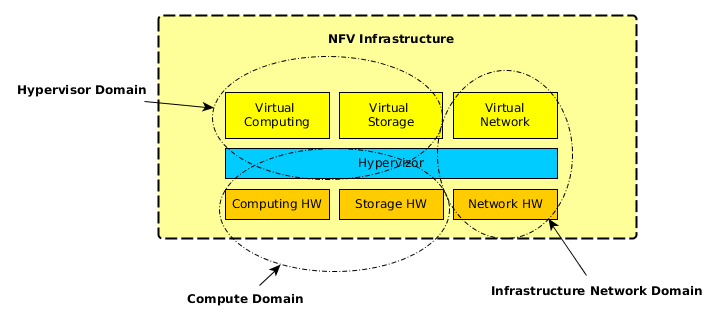
\includegraphics[scale=0.65]{images/infrastruktura}
\par\end{centering}
\caption{Schéma NFV infrastruktury\label{fig:infrastruktura}}
\end{figure}

Dá se říci, že referenční návrh infrastruktury pro NVF je podobný jako pro návrh infrastruktury pro cloud computing platformu. Měl by se tedy skládat z generických a komerčně vysoce dostupných serverů, které by měli být zapojeny do switche a tím by měla být zajištěna konektivita. Na tyto servery je následně nasazen jeden z dostupných hypervisorů. Výběr správného hypervisoru, které jsou v současné době dostupné na trhu, je hlavní podmínka správného a funkčního návrhu této části NFV frameworku. Přehled hypervisorů je uveden v kapitole \ref{sub:Hypervisor}. V produkčním prostředí by součástí řešení bylo samozřejmě řešení síťového návrhu. Tato práce však má sloužit pouze jako ukázka a z tohoto důvodu zde nebude síťový návrh zmíněn.

\subsection{Virtuální síťová funkce}

Virtuální síťová funkce (VNF) je dle \cite{NFV_VNF} určitá síťová funkce, která běží na NVF infrastruktuře a je zároveň NVF frameworkem řízena a spravována. Zároveň musí mít dobře definované rozhraní k ostatním síťovým funkcím, k VNF Managerovi a měla by obsahovat management rozhraní či port. Jedna VNF může být být obsažena v jednom virtuálním stroji nebo může být roztažena přes více virtuálních strojů. 

Na obrázku č. \ref{fig:VNF} je vidět jednoduché schéma virtuální síťové funkce dle referenčního návrhu \cite{NFV_VNF}. Celý životní cyklus VNF, což je vytvoření, spuštění, zastavení, smazání a škálování, řídí VNF Manager, který je součástí NVF managementu a orchestrace. Současně je možné dynamicky změnit aktuální konfiguraci pomocí Entity manageru (EM) přes management interface. EM může spravovat více VNF nebo právě jednu. Vnitřní struktura celé instance může být tvořena více komponentami (VNFC), které spolu mohou být navzájem provázány. Toto provázání však nemusí být viditelné zvenčí.

\begin{figure}[h]
\begin{centering}
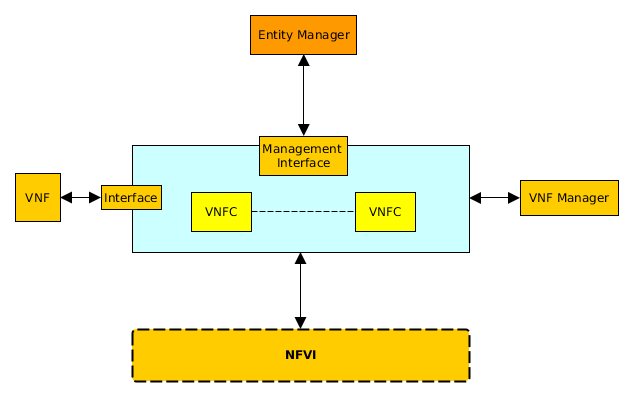
\includegraphics[scale=0.67]{images/VNF}
\par\end{centering}
\caption{Schéma virtuální síťové funkce\label{fig:VNF}}
\end{figure}

Pohledem na současný trh zjistíme, že VNF je prakticky poskytována ve 3 základních podobách.

\begin{itemize}
\item Softwarová aplikace - V tomto případě je poskytována VNF jako aplikace, která může být nainstalována na běžný operační systém jako je například GNU/Linux.
\item Ucelený operační systém - Zde je poskytován přímo celý operační systém, který může být nainstalován do virtuálního stroje nebo i na fyzický server.
\item Kompletní VM - Poskytovatel VNF může dát k dispozici rovnou přetvořený obraz virtuálního stroje (image), který může obsahovat operační systém se síťovými funkcemi. Tento systém však nemusí být klasicky dostupný operační systém jako je GNU/Linux či FreeBSD, ale může se jednat o speciálně vytvořený systém od výrobce. Tento způsob budou využívat poskytovatelé, kteří mají proprietární řešení pro síťová řešení jako je například Cisco či Juniper.
\end{itemize}

\subsection{Management a orchestrace NFV}

Management a orchestrace virtualizace síťových funkcí (NFV MANO) je nejdůležitější část celého NFV frameworku. Je tomu tak, protože MANO zajišťuje správné fungování NFV infrastruktury i jednotlivých virtuálních síťových funkcí. MANO také poskytuje funkce nutné pro provisioning VNF a související operace, jako je jejich konfigurace jednotlivých VNF a infrastruktury, na které běží. Zároveň spravuje a řídí životní cyklus fyzických a virtuálních zdrojů, které slouží pro podporu VNF. 

\begin{figure}[h]
\begin{centering}
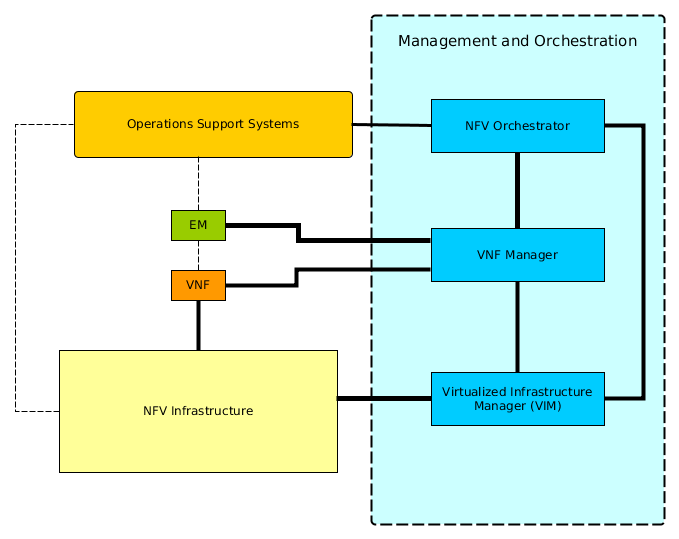
\includegraphics[scale=0.65]{images/MANO}
\par\end{centering}
\caption{Schéma NFV MANO\label{fig:MANO}}
\end{figure}

Jak vyplývá z obrázku č. \ref{fig:MANO}, tak referenční návrh MANO dle \cite{NFV_MANO} se skládá ze hlavních 3 částí, které se zabývají správnou jednotlivých vrstev NFV frameworku.

\begin{itemize}

\item Virtualized infrastructure manager (VIM) - Řídí a spravuje fyzické a virtuální zdroje v jedné doméně infrastuktury. Celková infrastruktura se může skládat z více domén a každá musí mít svůj VIM. Jeho typickými úlohami jsou vytvýření, udržování a uvolňování VM na dostupných zdrojích v doméně. Zároveň musí mít přehled o všech těchto a stavu hardwarových zdrojů.

\item VNF manager - Dohlíží na lifecycle management jednotlivých VNF instancí. To znamená, že výtváří, udržuke a ukončuje VNF instance, které běží na jednotlivých VM (ty však spravuje VIM). Opět může existovat více VNF managerů, kteří mohou spravovat jednu či více VNF.

\item NFV orchestator - Zjednodušeně slouží jako řízení a správu všech VIM a všech VNF managerů. Pomocí komunikace s VIM dokáže spravovat dostupné zdroje a pomocí komunikace s VNF managery dokáže řídit síťové služby. Jeho další funkcí je i přehled všech dostupných VNF, neboli katalog VNF, a registrace nových VNF do tohoto katalogu. Ten je pak dostupný uživatelům.
\end{itemize}

Celý systém je navržen tak, že by měl pracovat společně se stávajícími aplikacemi a systémy, které potencionální uživatelé používají pro provoz své infrastruktury a podnikových procesů (Operation support system).

V oblasti NFV MANO probíhá v součastnosti rozsáhlí vývoj a existuje několik projektů, které se tím zabývají. V článek \cite{NFV_orchestration} je nabídnut zajímavý přehled.

//TODO TOSCA 
\subsubsection{TOSCA}

\section{Možné technologie pro řešení}

V předchozí části byla popsána referenční architektura, kterou navrhla ETSI. V té jsou specifikovány funkční požadavky a nastíněny potřebná rozhraní. Přesto lze tento návrh považovat za poněkud omezený v rozsahu. Není v něm například definována řízení a správa starších zařízení, což může velice zkomplikovat provoz síťové infrastruktury, která se skládá z VNF i těchto starších zařízení. Kromě toho standardy a referenční implementace VNF, infrastruktury, a MANO prozatím nejsou k dispozici.

Z tohoto důvodu následuje návrh možnosti pro každou z oblastí architektury, které v současnosti mohou sloužit jako její řešení.


\subsection{Hypervisory} \label{sub:Hypervisor}

hypervisor je základná součástí cloudové platformy a frameworku pro virtualizaci síťových funkcí. Na trhu již existuje celá řada různých hypervisorů. Zde je uveden stručný přehled těch nejpoužívanějších.

\begin{itemize}
\item XEN - Je to hypervisor prvního typu, který pracuje na nejnižší vrstvě. Tato vrstva podporuje jeden nebo více hostovaných operačních systémů. První hostovaný systém se nazývá doménou 0 a slouží k přímému přístupu k hardwaru a jeho management. Do tohoto systému následně je možné přidávat další uživatelské domény, které mohou být linuxové systémy či Microsoft Windows.
\item KVM - Jedná se o virtualizaci založenou na linuxovém jádru. Každá virtuální instance má svůj vlastní virtualizovaný hardware včetně síťové karty, disku a grafické karty. Tento typ hypervisoru vyžaduje pro správnou funkci procesor s rozšířením pro virtualizaci hardwaru.
\item Microsoft Hyper-V - Zde se jedná o hypervisor od společnosti Microsoft, který lze nalézt v Windows Serverech od verze 2008. Hyper-V je hypervisorově stavěný serverový systém. To znamená, že má svůj hlavní operační systém a pomocí virtualizace se skrze něj mohuo spustit další operační systémy. 
\item WMware ESXi - Varianta  ESXi  je  odlehčená  verze ESX  klienta,  která  dovoluje  běžet  hostitelský systém na výměnném zařízení. Jde o tenký klient s vlastním linuxovém jádrem, který běží přímo nad hardwarovou vrstvou. Kernel ESXi funguje jako hostitelský operační systém pro vrstvení dalších služeb. Kernel na sebe váže modul vmkernel s dalšími obslužnými funkcemi, který tvoří základní stavební kámen celého řešení. Výhodou tohoto řešení  je možnost alokace co  největšího  množství  hardwarových prostředků  pro hostované systémy.  Tenký  klient  totiž  zbytečně nevyužívá  systémové prostředky  hostujícího  serveru.

\end{itemize}

\subsection{VNF}

Pokud se podíváme na trh s VNF u některých vendorů, tak zjistíme, že mnozí poskytují virtuální instance, které se dají použít pro účely VNF v této práci. Tato práce je zaměřena především na funkce firewallu a proto zde jsou uvedeny příklady pouze pro ně. Uvedeny jsou hlavně produkty největších a nejpoužívanějších poskytovatelů síťových prvků a také open-source firewall.

\begin{itemize}
\item Juniper vSRX - Jde o firewall od společnosti Juniper, který je obdobou jejich fyzického zařízení Juniper SRX. Jde virtuální instanci poskytující funkce pro firewall, routing a pokročilé bezpečností funkce pro poskytovale telekomunikačních služeb a větší společnosti. Toto VM je určené pro privátní, public i hybrid cloud. 
\item Fortigate-VM - Fortigate Virtual Appliances je řešení pro cloudové prostředí od společnosti Fortinet. Nabízí stejně funkce pro firewall jako jsou obsaženy ve Fortigate fyzických zařízeních.
\item Cisco ASAv - Společnost Cisco nabízí Adaptive Security Virtual Appliance (ASAv), která obsahuje stejný software jako fyzické ASA zařízení a vetšinu funkcí pro firewall, routing a VPN. 
\item PFSense - PFSense je open-source projekt, který má za cíl poskytnout firewall postavený na operačním systému FreeBSD, který může běžet na klasické architektuře jednodeskových počítaču. Toto řešení poskytuje všechny důležité vlastnosti komerčních firewallů, má jednoduché ovládání a je to otevřené řešení.
\end{itemize} 

\subsection{Cloud platforma}

Pro účely vytvoření infrastruktury, a vůbec možnost využití NFV v datovém centru, je nutná cloudová platforma. Existují několik řešení, které lze pro tyto účely použít. Dvě z nejčastějších jsou OpenStack a VMware vCloud.


\subsubsection{OpenStack}

OpenStack je open-source platformou umožňující postavit IaaS cloud, který může být nainstalován i na běžném hardwaru. Toto řešení má za cíl vytvořit dostupnou cloudovou platformu, která bude splňovat všechny potřeby privátních a veřejných cloudů nezávisle na velikosti řešení. \cite{OpenStack}

Celá stavba systému OpenStack se skládá z několika na sobě nezávislých projektů (modulů), které řeší různé oblasti cloudové platformy. Tyto projekty mezi sebou komunikují pomocí otevřených API a mohou být spravovány pomocí dashboardu. Celé administrace OpenStacku může být prováděna přes webově rozhraní, příkazovou řádku či přímo pomocí příkazů zaslaných do API. Celé toto řešení se vyznačuje jednoduchostí implementace, škálovatelností a rychlým vývojem nových vylepšení. Hlavními moduly OpenStacku jsou \cite{OpenStack} \cite{OpenStack2}:

\begin{itemize}
\item Keystone - identifikační služba používaná OpenStackem pro autorizaci a autentizaci. Ověřování probíhá pomocí tokenů. Uživatel přihlášením odesílá žádost na Keystone, který tento modul zpracuje, zjistí pověření a vytvoří token. Vytvořený token je poté odesílán s žádostí do ostatních služeb. Zde dojde ke komparaci tokenu se současnou přístupovou politikou a dojde ke zjištění, zdali má uživatel dostatečná oprávnění pro provedení požadovaného úkonu.
\item Glance - služba umožňující práci s virtuálními diskovými obrazy (imagy). Tyto obrazy mohou být uloženy na mnoha různých místech od lokálních systémových disků až po distribuované souborové systémy, jako je OpenStack Storage.
\item Nova - tento modul poskytuje výpočetní služby. Umožňuje tedy běh několika instancí virtuálních strojů na několika hostitelských strojích, nan kterých je nainstalována služba OpenStack compute. OpenStack podporuje hypervizory KVM, QEMU, VMware ESX, Hyper-V, Xen. 
\item Neutron - je služba pro správu všech síťových aspektů OpenStacku. Jedná se tedy o SDN komponentu. Neutron podporuje možnost rozšíření o tzv. pluginy, které umožňují využívat řešení třetích stran pro síťování.
\item Cinder - poskytuje infrastrukturu pro mapování volumů v OpenStacku.
\item Ceilometer - služba, která sbírá měřená data a monitoruje tak využívané zdroje.
\item Heat - umožňuje automatizovanou orchestraci virtuálních strojů na základě vytvořených templatů.
\item Horizon - představuje dashboard, který umožňuje cloudovým administrátorům a uživatelům spravovat různé zdroje a služby OpenStacku. Dashboard umožňuje interakci s OpenStackovým kontrolerem prostředníctvím API. 
\end{itemize}

\subsubsection{VMware vCloud}

Společnost Vmware poskytuje pro privátní cloudové systémy své řešení, které označuje jako VMware vCloud. Toto řešení je poskládané z jednotlivých produktů této společnosti. Celá architektura má hierarchická model, který je vidět na obrázku č. \ref{fig:vmware}

\begin{figure}[h]
\begin{centering}
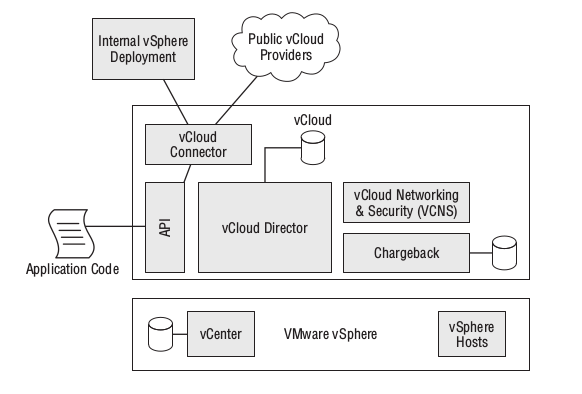
\includegraphics[scale=0.65]{images/vmware}
\par\end{centering}
\caption{Schéma VMware vCloud, převzato z \cite{vmware}\label{fig:vmware}}
\end{figure}

Dle \cite{vmware} se VMware vCloud skláda především z těchto komponent.

\begin{itemize}
\item VMware vCloud Director - je  jedna  ze základních součástí potřebných pro vytvoření  privátního  cloudu ve stylu VMwaru.  Umožňuje vytvořit  a  doručovat  koncovým  zákazníkům infrastrukturu jako službu. Je propojen a přímo spolupracuje s VMware vSphere center.
\item VMware vSphere - tento produkt slouží pro vytvoření virtualizované infrastruktury. Je to sdružení více komponent. Ty nejhlavnější jsou:

\begin{itemize}
\item VMware ESX (ESXi) - hypervisor, který byl popsán v kapitole \ref{sub:Hypervisor}.
\item VMware vCenter Server - umožňuje efektivní a pokročilejčí správu virtualizovaného prostředí, bez ohledu na jeho velikost. Jedná se např.o snadné vytváření nových virtuálních počítačů, jejich  klonování  nebo  importování  z jiného  úložiště.  
\item VMware vSphere Client - je určený pro dálkovou správu hostitelů ESXi. Připojit se můžeme prostřednictvím vCenter serveru nebo přímo přes ESXi server.
\end{itemize} 
\item VMware vCloud Networking and Security - poskytuje síťování a bezpečnost pro vituální prostředí. Poskytuje mnoho síťových funkcí a poskytuje framework pro integraci řešeí třetích stran.
\item VMware vShield - představuje možnost zabezpečení v prostředí VMware VSphere. Může být konfigurován pomocí vShield Managera, který umožňuje centrální správu přes webové rozhraní, vSphere klient plug-in, nebo command line interface (CLI).
\item VMware vCenter Chargeback - slouží pro monitorování virtuálních strojů, které následně může být účtováno.
\end{itemize}

\subsection{SDN}

Součástí řešení pro datové centrum je dnes i SDN. I zde existuje několik možností. Dvě z nejpoužívanější řešení jsou:

\subsubsection{OpenContrail} 

OpenContrail je systém, který může být použit v mnoha síťových scénářích jako například v cloud networkingu nebo v sítích poskytovatele síťových služeb. V privátním cloudu, ve Virtual Private Cloud (VPC) a v IaaS se vyskytuje prostředí s velkým množstvím tenantů, kde několik tenantů sdílí stejné fyzické zdroje (server, uložiště, fyzickou síť). Každý tenant má přiřazeny vlastní logické zdroje (virtuální stroje, virtuální uložiště, virtuální sítě). Tyto logické zdroje různých tenantů musí být od sebe odděleny. Virtuální sítě v datacentrech mohou být také spojeny s fyzickou IP VPN nebo L2 VPN. \cite{OpenContrail}

OpenContrail je složen ze dvou hlavních komponent. První z nich je Controller, který je logicky centralizovaný, ale fyzicky distribuovaný. To znamená, že je složen z několika typů rolí a každý z nich má několik instancí z důvodu vysoké dostupnosti a horizontální škálovatelnosti. Tyto role mohou být fyzické servery nebo virtuální stroje. Tyto role jsou \cite{OpenContrail2}: 

\begin{itemize}
\item Configuration role - poskytuje north-bound REST API. Toto API může být použito pro konfiguraci systému nebo pro extrahování operačního stavu systému.
\item Control role - implementuje logicky centralizovanou část control planu.
\item Analytics role - je zodpovědný za sběr, porovnání a prezentaci analytických informací.
\end{itemize}

Další komponentou je vRouter, který má na starost přenos dat. VRouter běží na virtualizovaném serveru, na kterém běží hypervizor. Rozšiřuje fyzickou síť v datovém centru o virtuální overlay síť hostovanou ve virtualizovaných serverech. VRouter narozdíl od vSwitchů poskytuje směrování a služby vyšších vrstev. Data plane, tedy vRoutery mezi sebou, může používat různé technologie overlay jako MPLS over GRE, MPLS over UDP a VXLAN. Control plane protocol mezi Controllerem a fyzickým gateway routerem (nebo switchem) je BGP. Protokol používaný mezi Controllerem a vRoutery se nazývá XMPP. Obrázek č. \ref{fig:contrail} ukazuje schéma OpenContrailu.

\begin{figure}[h]
\begin{centering}
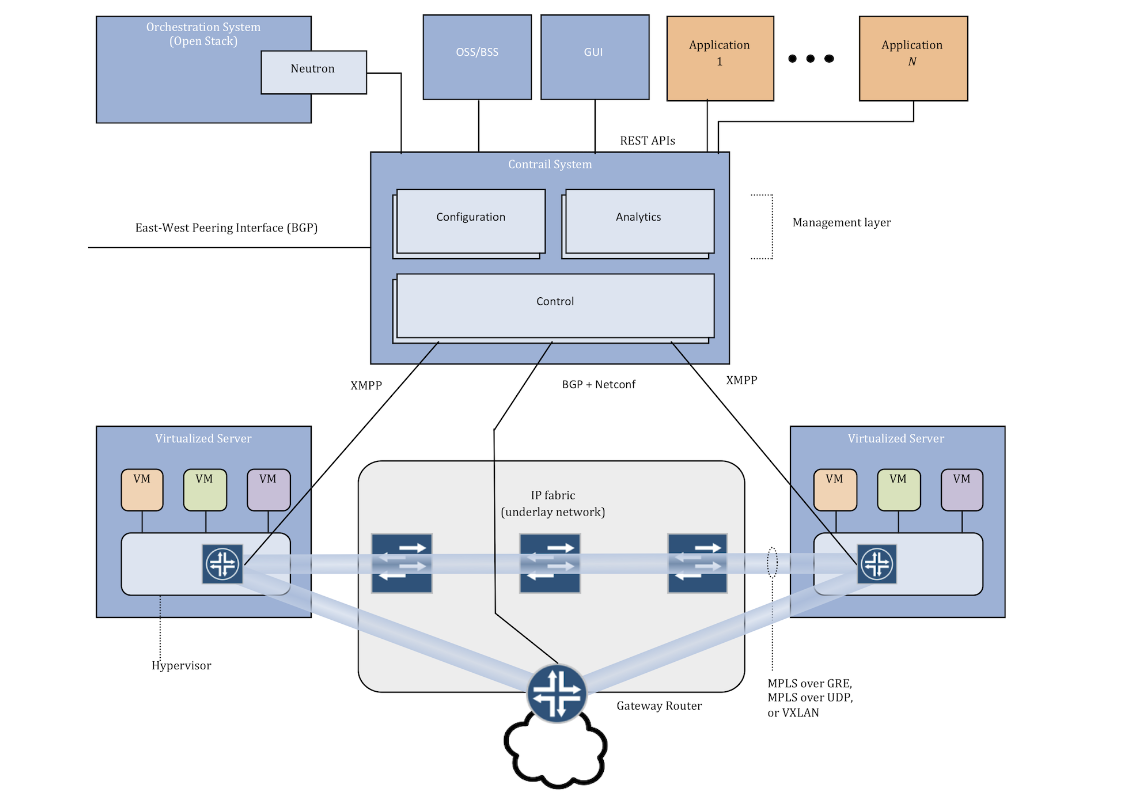
\includegraphics[scale=0.35]{images/contrail}
\par\end{centering}
\caption{Schéma OpenContrail, převzato z \cite{OpenContrail}\label{fig:contrail}}
\end{figure}

\subsubsection{VMware NSX}

VMware NSX představuje technologii síťové virtualizace od společnosti VMware. NSX umožňuje vytváření a správu softwarových virtuálních sítí napříč celým datovým centrem. Architektura NSX je složená z Consumption, Management plane, Control plane a Data plane. \cite{VMware_NSX}

\begin{itemize}
\item Data plane - je představován virtuálními switchi, jako je NSX vSwitch či Open vSwitch. 
\item Control role - zde je komponentou NSX controller či jejich cluster. NSX controller přijímá instrukce, na konfiguraci logických sítí od tenantů, prostřednictvím NSX API. Poté pomocí OpenFlow konfiguruje vSwitche.
\item Management plane a Consumption - je tvořen NSX managerem, který poskytuje centralizovanou možnost konfigurace a REST API. \cite{VMware_NSX}
\end{itemize}

U tohoto řešení existují dva pohledy na síťovou infrastrukturu. První je transportní, který představuje underlay síť. Ta se skládá z síťový hardwaru propojující hypervizory. Druhý pohled je logický. Ten představuje množinu síťových služeb, které vidí každý tenant či virtualizovaný stroj v tomto tenantu. V multi-tenant prostředí má každý tenant svůj vlastní logický pohled na svoji síť a nemůže vidět sítě ostatních tenantů. \cite{VMware_NSX}

VMware NSX je dostupný ve dvou verzích - NSX-v a NSX-mh. NSX-v je verze závislá na proprietárním VMware řešení, tedy spolupracuje pouze s hypervizorem vSphere od VMware. Druhá verze je NSX-mh, kde mh znamená multi hypervizor a je tedy možné použití s různými hypervizory. 